\chapter{Preguntas adicionales}
\section{Examen de prueba: Autoevaluación del curso}
\subsection{Exercise 1}
We have a sequence 5241977 bases long. Table below shows the sequence statistics.

\begin{table}[htbp]
\centering
\begin{tabular}{l | l l l l l }
& overall & from A & from C & from G & from T \\ \hline
to A & 0.247 & 0.296 & 0.277 & 0.229 & 0.187 \\
to C & 0.253 & 0.223 & 0.231 & 0.323 & 0.235 \\
to G & 0.252 & 0.208 & 0.289 & 0.230 & 0.281 \\
to T & 0.247 & 0.273 & 0.202 & 0.218 & 0.298
\end{tabular}
\end{table}

How many TATA-box motifs (TATAAT) would you expect by chance according to a simple multinomial model?
$$ 0.247^6 \cdot 5241977 = 1190.36 \approx 1190 $$

And according to a Markov-chain model where the initial prob. is the same as overall one?
$$0.247 \cdot 0.187 \cdot 0.273 \cdot 0.187 \cdot 0.296 \cdot 0.273 \cdot 5241977 = 998.83 \approx 999 $$

\subsection{Exercise 2}
The following contains a python function that accepts a DNA sequence and returns the data structure AbsdiNucl\_freq containing the absolute frequencies of dinucleotides. 

\begin{lstlisting}
## Function to count absolute dinucleotide frequencies
def AbsdiNuclFrq(Seq):
	# Initializes a dictionary for all 16 potential dinucleotides
	AbsdiNucl_freq = {}
	for Base1 in ["A", "C", "G", "T"]:
		for Base2 in ["A", "C", "G", "T"]:
			AbsdiNucl_freq[Base1+Base2] = 0
	# count frequencies
	for pos in range(0, len(Seq) - 1):
		if Seq[pos:pos+2] in AbsdiNucl_freq.keys():
			AbsdiNucl_freq[Seq[pos:pos+2]] = AbsdiNucl_freq[Seq[pos:pos+2]]+1
	# Sequence length
	return(AbsdiNucl_freq) #return a identifier-null dict.
\end{lstlisting}

Which of the following expressions would you use to retrieve the frequency of the dinucleotide GC? \textbf{Since the frequencies are stored in a dictionary, we can just index by the dinucleotide we are interested in, so: AbsdiNucl\_freq["GC"]}

\subsection{Exercise 3}
The following figure shows several Dot-Matrix obtained from the alignment of different combinations of the indicated protein sequences or the indicated DNA sequences. Indicate which sequences were aligned in each case.
\begin{figure}[htbp]
\centering
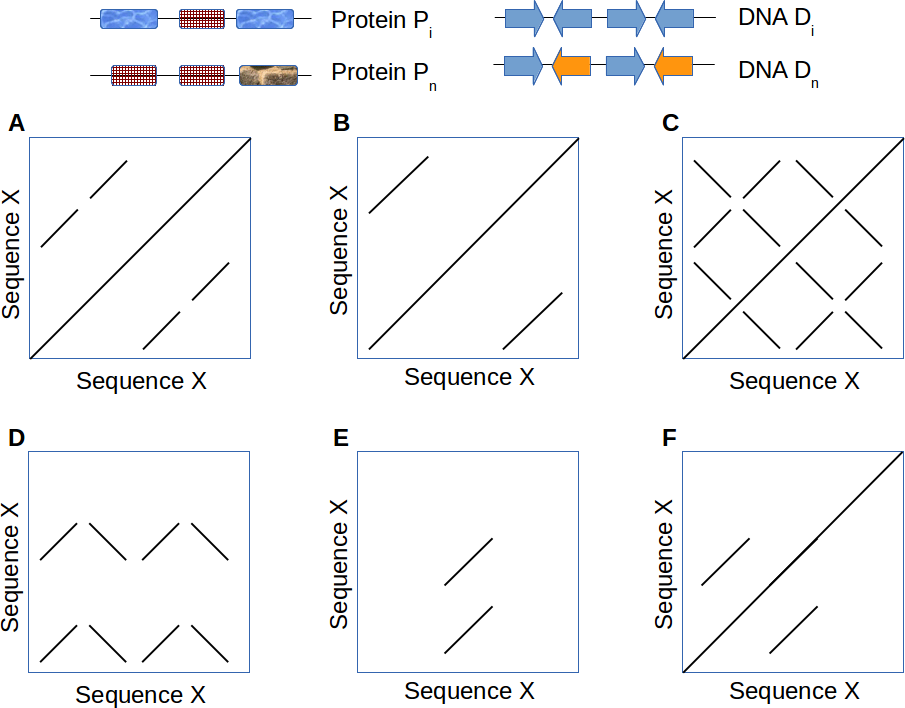
\includegraphics[width = 0.7\textwidth]{figs/exam-ex3.png}
\end{figure}

Trick: when a sequence is aligned with itself, there is a whole diagonal in the dot matrix.

\noindent
Dot-Matrix A: DNA Dn vs DNA Dn \\
Dot-Matrix B: Protein Pi vs Protein Pi \\
Dot-Matrix C: DNA Di vs DNA Di\\
Dot-Matrix D: DNA Di vs DNA Dn \\
Dot-Matrix E: Protein Pi vs Protein Pn \\
Dot-Matrix F: Protein Pn vs Protein Pn \\

\subsection{Exercise 4}
Indicate the optimal method to apply in the following situations:
\begin{enumerate}
\item Protein search against a database to identify similar proteins: \textbf{BLAST}
\item  You are interested in finding conserved domains within a set of given sequences: \textbf{Smith-Waterman - local alignment}
\item You need the best alignment between the whole extension of two proteins: \textbf{Needleman-Wunsch - global alignment}
\item Quick identification of repeated sequences between two chromosomes: \textbf{Dot-Matrix}
\end{enumerate}

\subsection{Exercise 5}
We performed a pairwise alignment between the human HRAS and the indicated \textit{C. elegans} proteins using BLAST(p) with default parameters and got the indicated scores. The figure shows the probability density (graphs on top) and cumulative probability (bottom graphs) for the BLAST score values for random alignments under these conditions (graphs on the right are just a zoom of the left graphs on the values 30 to 90). The red lines mark the position of problem scores. Indicate the probability of getting an alignment with an associated score equal or higher than these just by chance (choose the one that best describes it):

\begin{figure}[htbp]
\centering
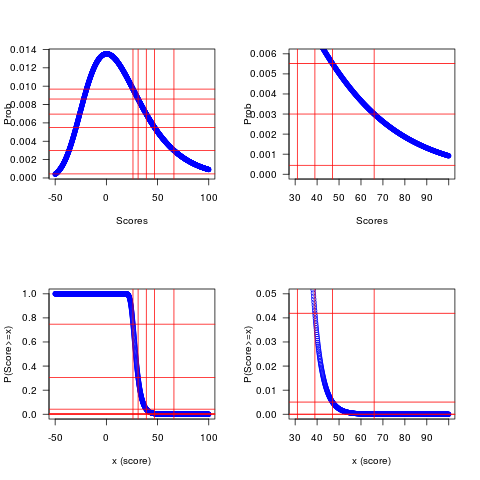
\includegraphics[width = 0.7\textwidth]{figs/exam-ex5.png}
\end{figure}

For this problem we have to use the cumulative probabilities (bottom graphs):
\begin{enumerate}
\item  KBRAS, score=120. p-value: \textbf{<0.001}
\item ARL2, score=66. p-value: \textbf{<0.001}
\item CKI1, score=47. p-value: \textbf{<0.01}
\item MED20, score=39. p-value: \textbf{<0.05}
\item ZK688, score=31. p-value: \textbf{>0.05}
\item RL15, score=26. p-value: \textbf{>0.05}
\end{enumerate}

\subsection{Exercise 6}
To generate the alignment between two sequences (of length m and n) using dynamic programing we follow these steps:
\begin{enumerate}
\item  Fill a m*n matrix with the scores resuting from: 
$$ Score = Max 
  \begin{cases}
    F(i-1, j-1) + s(x,y)\\ 
    F(i-1, j) - GapPenalty \\
    F(i, j-1) - GapPenalty
  \end{cases}
$$
  
\item  Reconstruct the alignment. Starting from bottom-right cell of the matrix generated in \#1 trace-back the pointers to the initial top-left cell.
\end{enumerate}

The pseudocode for this algorithm is depicted here:
\begin{figure}[htbp]
\centering
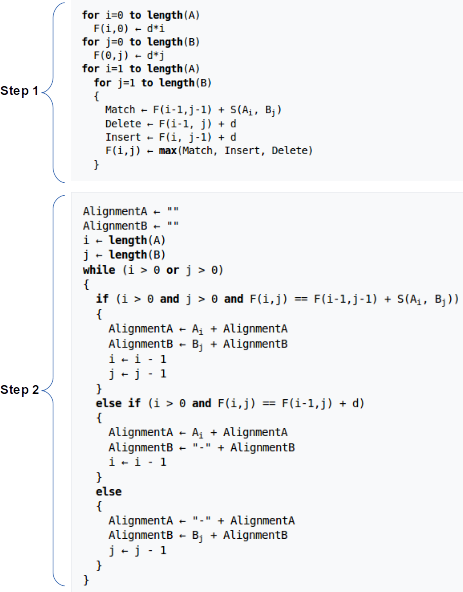
\includegraphics[width = 0.5\textwidth]{figs/exam-ex6.png}
\end{figure}

Are the pointers saved during the generation of the matrix (step 1)? \textbf{NO}

\subsection{Exercise 7}
Big-O notation is used to: \textbf{describe concisely the running time of an algorithm.}

\subsection{Exercise 8}
Match the following MSA with the simplest model that preserves most of the information in that alignment. keeping in mind that you can choose each model only once.
\begin{figure}[htbp]
\centering
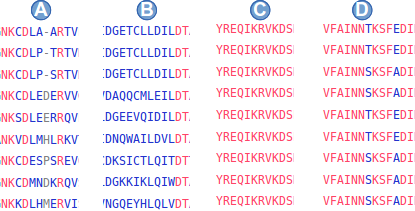
\includegraphics[width = 0.7\textwidth]{figs/exam-ex8.png}
\end{figure}

\noindent
Alignment A: \textbf{Hidden Markov Model (HMM)} \\
Alignment B: \textbf{Position Specific Scoring Matrix (profile) (PSSM)} \\
Alignment C: \textbf{Consensus sequence} \\
Alignment D: \textbf{Regular expression (pattern)}

Los modelos ordenados por orden de complejidad ascendente son secuencia consenso, patrón, PSSM y HMM. Con eso, solo es cuestión de ordenar los alineamientos por complejidad y asignar el modelo.

\subsection{Exercise 9}
We have aligned several tyrosine protein kinases and found a conserved region corresponding to the active site of these enzymes. Here is the regular expression representing this alignment: [LIVMFYC]-{A}-[HY]-x-D-[LIVMFY]-[RSTAC]-{D}-{PF}-N-[LIVMFYC] 

\begin{figure}[htbp]
\centering
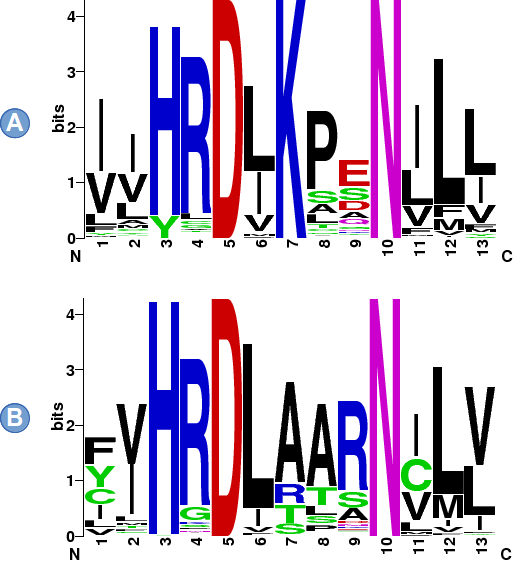
\includegraphics[width = 0.4\textwidth]{figs/exam-ex9.png}
\end{figure}

Which of the sequence logos in the figure represent this alignment? \textbf{B} \\
Which of the following positions shows the lowest information content in that alignment? \textbf{Position 1}

\subsection{Exercise 10}
Commonly used MSA programs: \textbf{use an heuristic approach composed of three steps: distance calculation, dendrogram tree generation, pairwise alignment based on tree topology.}

BLAST uses  an heuristic approach composed of three steps (construction of a word list from the sequences, identification of identical words (seeds), extension of seeds) for the search of a sequence within a database. 

Global and local alignments between two sequences  use an extension of dynamic programming to generate the alignment.

\section{Preguntas anteriores}
\subsection{Exercise 1}
You have access to a fragment of the genome of a new ssDNA virus. We assume it is a representative fragment and that the composition is homogeneous throughout the genome. The frequencies of bases in this sequence fragment are given in the table below. Use Maximum Likelihood (ML) to estimate the following parameters of a basic multinomial model and a Markov-chain model for this sequence:

Multinomial model, probability of A, $P_A = \frac{1}{4} = 0,25 $

\begin{table}[htbp]
\centering
\begin{tabular}{l | l l l l }
& from A & from C & from G & from T \\ \hline
To A & 21 & 37 & 41 & 25 \\
To C & 21 & 62 & 58 & 17 \\
To G & 35 & 50 & 26 & 27 \\
To T & 47 & 11 & 13 & 9
\end{tabular}
\end{table}

Markov-model probability of transition from T to A, $P_{TA} = \frac{from T to A}{from T to everything} = \frac{25}{25 + 17 + 27 + 9} = 0.3205$

\subsection{Exercise 10}
According to data in the figure, the observed mutation frequency Met/Arg is the same as Phe/Asn. What about their corresponding entries in the BLOSUM62 substitution matrix?

\begin{figure}[htbp]
\centering
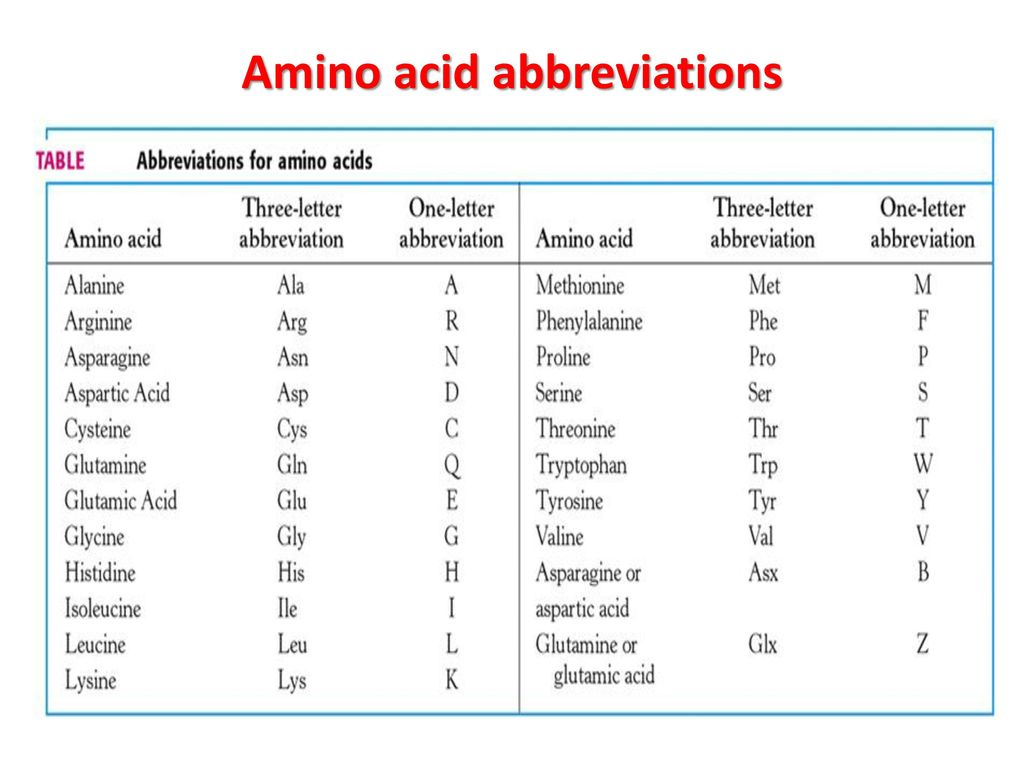
\includegraphics[width = 0.7\textwidth]{figs/aa_abbreviations.png}
\end{figure}

The observed mutation frequency is 8/10000. For the entry in the BLOSUM62 substitution matrix ($2 \cdot log_2 (odds ratio) = 2 \cdot log_2 (\frac{observed}{expected}$):
$$S_{M, R} = 2 \cdot log_2 (\frac{8/10000}{0.025 \cdot 0.052}) = -1.4 \approx -1$$
$$S_{F, N} = 2 \cdot log_2 (\frac{8/10000}{0.047 \cdot 0.045}) = -2.8 \approx -3$$
In conclusion, \textbf{Met/Arg have higher entry value than Phe/Asn}.

If all the entries in the diagonal of the mutation frequency table were the same, what would be their corresponding entry in the scoring matrix? \textbf{If the observed value would be the same for the entire diagonal, their values for the scoring matrix would be determined by their expected values. W has the lowest expected value and would therefore have the highest value in the scoring matrix.}

\begin{figure}[htbp]
\centering
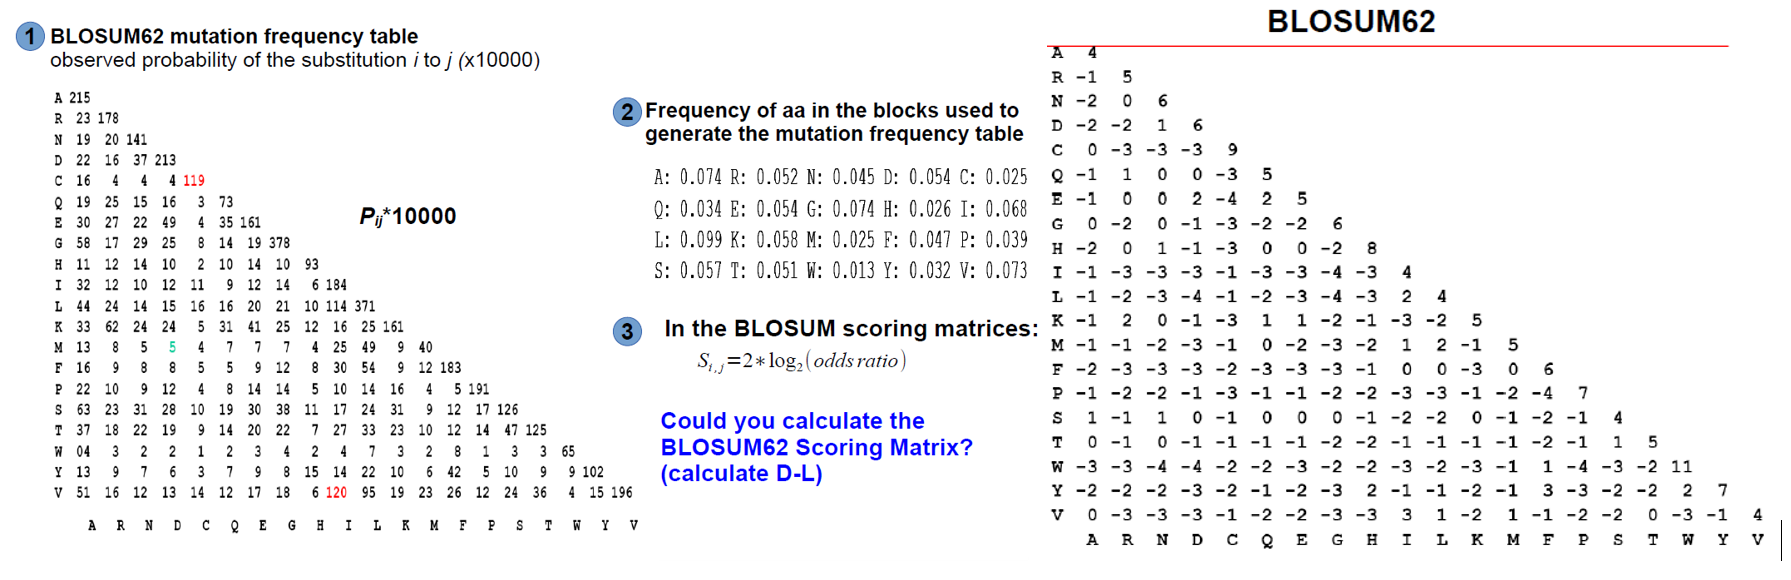
\includegraphics[width = \textwidth]{figs/ejercicio-blosum.png}
\end{figure}

\subsection{Exercise 12}
We performed a BLAST search using a human protein (X) as query against all \textit{Caenorhabditis elegans} proteins and got several hits. The figure below shows two of them.

\begin{figure}[htbp]
\centering
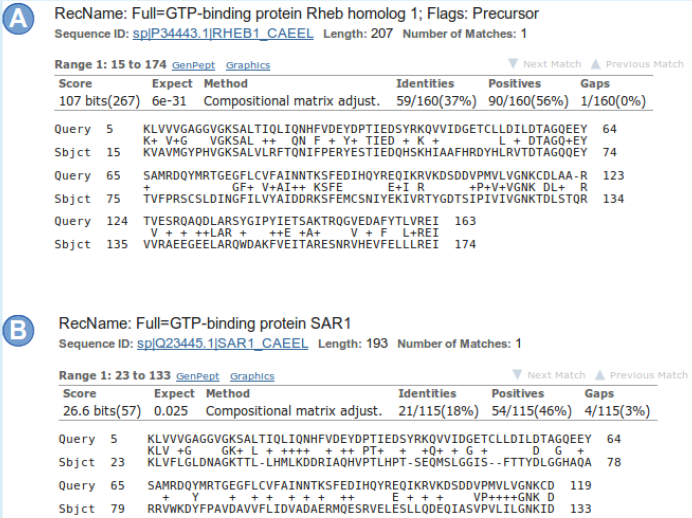
\includegraphics[width = 0.5\textwidth]{figs/exam-ex12.png}
\end{figure}

Indicate which of the following statements are correct:
\begin{enumerate}
\item Protein X and B share less than 25\% identity: \textbf{True, 18\%}
\item Protein X and A share a 37\% homology: \textbf{False, they are homologs, but this cannot be calculated on percentage; 37\% is the identity, not homology.}
\item Protein X and A are very likely to be homologs: \textbf{True, from 30\% identity onwards it can be considered as homology.}
\item Protein X and B are likely to have similar function/structure: \textbf{False}
\end{enumerate}

\subsection{Exercise 13}
Indicate which algorithm is best suited to solve the following alignments:
\begin{enumerate}
\item Alignment of two proteins that I suspect only share a short domain (I need to get the actual alignment): \textbf{Smith-Waterman's local alignment}.
\item A simple way to explore if a sequence contains duplicated regions: \textbf{Dot-matrix}
\item I need the optimal (best possible) alignment between two sequences: \textbf{Needleman-Wunsch's global alignment with dynamic programming}
\item Compare a protein sequence agains a large database in a short time: \textbf{word-based heuristic algorithm like BLAST}
\end{enumerate}

\subsection{Exercise 14}
What is the minimum number of permutations (minimum number of score values from random alignments) that we would need to determine if a given score has an associated p-value of <0.001? \textbf{ 1000 permutations, since 0.001 = 1/1000}

\subsection{Exercise 16}
What is the uncertainty (in bits) about the nucleotide residue occupying at a given DNA position? \textbf{2}. 
\begin{figure}[htbp]
\centering
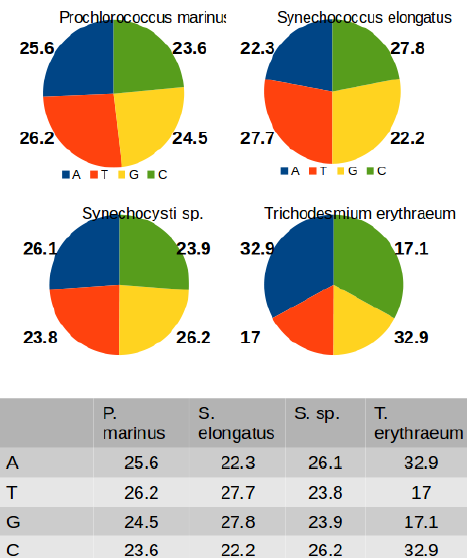
\includegraphics[width = 0.3\textwidth]{figs/exam-ex16.png}
\end{figure}
What is the entropy for a random position in the cyanobacteria genomes depicted in the figure?
\begin{itemize}
\item P. marinus: $-(0.256 \cdot log_2 (0.256) + 0.236 \cdot log_2(0.236) + 0.262 \cdot log_2 (0.262) + 0.245 \cdot log_2(0.245)) =  1.998 $
\item S. elongatus: $-(0.223 \cdot log_2 (0.223) + 0.278 \cdot log_2(0.278) + 0.277 \cdot log_2 (0.277) + 0.222 \cdot log_2(0.222)) =  1.991 $
\item S. sp.: $-(0.261 \cdot log_2 (0.261) + 0.239 \cdot log_2(0.239) + 0.238 \cdot log_2 (0.238) + 0.262 \cdot log_2(0.262)) =  1.998 $
\item T. erythraeum: $-(0.329 \cdot log_2 (0.329) + 0.171 \cdot log_2(0.171) + 0.17 \cdot log_2 (0.17) + 0.329 \cdot log_2(0.329)) =  1.926 $
\end{itemize}

What is the maximum possible entropy for a position in a DNA molecule? \textbf{2}. With this in mind, how much information does the human genome hold (in bits)? $2 \cdot 3 \cdot 10^9 = 6,000,000,000$ and in MBytes? $6,000,000,000 / 8 = 750,000,000 bytes / 10^6 = 750 MBytes$

What is the maximum theoretical entropy for a position in a protein sequence (in bits)?  $- \sum_{1}^{20} (\frac{1}{20} \cdot log_2(\frac{1}{20})) = 4.322$

\subsection{Exercise 27}
Determine the average length of the restriction fragments produced by the six-cutter restriction enzyme Smal that cuts the restriction site CCCGGG. Consider the case of (a) a genome with C+G content of 70\% and (b) a genome with G+C content of 30\%. In both cases, assume that the genomic sequence can be represented by a multinomial model with probabilities of nucleotides such that pG = pC and pA = pT. 

What would be the average length of the restriction fragments in case (a)? 
C and G have in total 70\% probability, so each has 35\%. The probability of the fragment in the human genome would be $0.35^6 \cdot 3 \cdot 10^9 = 5514796.875$. This represents the number of times the restriction enzyme would cut. To get the length of each piece: $3 \cdot 10^9 / 5514796.875 = 543.99 \approx 544$

What would be the average length of the restriction fragments in case (b)? 
C and G have in total 30\% probability, so each has 15\%. The probability of the fragment in the human genome would be $0.15^6 \cdot 3 \cdot 10^9 = 34171.875$. This represents the number of times the restriction enzyme would cut. To get the length of each piece: $3 \cdot 10^9 / 34171.875 = 87791.495 \approx 87791$

\subsection{Exercise 29}
A 4200nt long DNA fragment from the genome of bacteria \textit{Bioquimicus sp.} was sequenced and the results used to estimate the parameters of a Markov Chain model representation of this DNA. The observed counts for the sixteen possible dinucleotides in the + strand are shown in the table below, where rows indicate the first nucleotide and columns the second nucleotide of the dinucleotide.

\begin{table}[htbp]
\centering
\begin{tabular}{l | l l l l }
& A & C & G & T \\ \hline
A & 510 & 380 & 210 & 190 \\
C & 240 & 170 & 360 & 230 \\
G & 370 & 200 & 220 & 210 \\
T & 190 & 170 & 220 & 220
\end{tabular}
\end{table}

Find the maximum likelihood estimates of the transition probabilities $P_{TT}$ and $P_{AG}$ of the Markov chain model of the positive strand of this DNA:
$$P_{TT+} = \frac{220}{220+220+170+190} = 0.275$$
$$P_{AG+} = \frac{210}{210+190+380+510} = 0.163$$

Find also the transition probabilities $P_{TT}$ and $P_{AG}$ of the Markov chain model of the negative strand of this DNA:
$$P_{TT-} = \frac{AA}{AA + CA + GA + TA} = \frac{510}{510+240+370+190} = 0.389$$
$$P_{AG-} = \frac{CT}{CT + AT + GT + TT} = \frac{230}{230+190+210+220} = 0.271$$

\subsection{Exercise 30}
Life has just been discovered in Mars. Interestingly, martian microbes have proteins composed only by three aminoacids (X, Y, Z). Scientists have been able to generate some alignments from related martian proteins and from them calculated the mutation frequency table shown below (P*60). To calculate the entries of the martian scoring matrix, use the formula $S_{i,j} = 2 \cdot log_2(odds ratio)$

\begin{table}[htbp]
\centering
\begin{tabular}{l l l l || l }
& X & Y & Z & freq \\ \hline
X & 28 &  &  & 0.58333 \\
Y & 8 & 6 &  & 0.25 \\
Z & 6 & 10 & 2 & 0.1666 \\
\end{tabular}
\end{table}

What would be the value for the entry for the X to Z substitution in the corresponding scoring matrix?
$$2 \cdot log_2(\frac{6/60}{0.58333 \cdot 0.1666}) = 0.082 \approx 0$$

What would be the value for the entry for the Y to Y substitution in the corresponding scoring matrix?
$$2 \cdot log_2(\frac{6/60}{0.25 \cdot 0.25}) = 1.356 \approx 1$$

If all the entries in the mutation table were the same (e.g. all of them were 10 corresponding to a mutation of 10/60), the entries in the scoring matrix would be the same: \textbf{False, since the amino acid mutation is different.}

\subsection{Exercise 204}
The logo MA0598 below represents the binding sites for the transcription factor EHF. How many EHF binding sites would you expect in the human genome assuming a multinomial model with equal frequencies for all four nucleotides?

\begin{figure}[htbp]
\centering
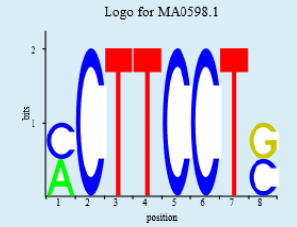
\includegraphics[width = 0.3\textwidth]{figs/exam-ex204.png}
\end{figure}

$$0.25^6 \cdot 0.5^2 \cdot 3 \cdot 10^9 = 183105.4688$$

\subsection{Exercise 203}
The sequence logo shown below was derived from the alignmed of 31 binding sites for the transcription factor XX. The matrix below the logo contains the number of nucleotides found at each position, but the columns have been shuffled so that the columns of the matrix (c1 to c6) do not necessarily correspond to each position in the logo (position 1 - 6). In addition, we do not know which nucleotide is recorded in each row of the matrix. Reconstruct the original order of columns in the matrix by matching the following terms:

\begin{figure}[htbp]
\centering
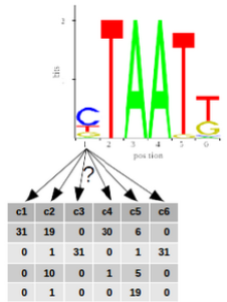
\includegraphics[width = 0.3\textwidth]{figs/exam-ex203.png}
\end{figure}

Positions 3 and 4 of the logo are the same, so we can conclude that they correspond to columns c3 and c6 of the matrix. Since these positions only have A, row 2 of the matrix has to represent A. Position 2 of the logo only has a T, which means that it must be column c1 and that row 1 is T. Position 1 of the logo contains all nucleotides, meaning that it can be either c2 or c5. However, the most frequent nucleotide is C, and since we know that row 1 is T, column c2 is excluded and c5 left (and row 4 must be C).

\begin{itemize}
\item Position 3 of the logo: \textbf{Column c6}
\item Position 1 of the logo: \textbf{Column c5}
\item Position 6 of the logo: \textbf{Column c2}
\item Row 2 of the matrix: \textbf{Counts for A}
\item Row 1 of the matrix: \textbf{Counts for T}
\end{itemize}